\chapter{Diseño e implementación} % Main chapter title

\label{Chapter3} % Change X to a consecutive number; for referencing this chapter elsewhere, use \ref{ChapterX}

\definecolor{mygreen}{rgb}{0,0.6,0}
\definecolor{mygray}{rgb}{0.5,0.5,0.5}
\definecolor{mymauve}{rgb}{0.58,0,0.82}

%%%%%%%%%%%%%%%%%%%%%%%%%%%%%%%%%%%%%%%%%%%%%%%%%%%%%%%%%%%%%%%%%%%%%%%%%%%%%
% parámetros para configurar el formato del código en los entornos lstlisting
%%%%%%%%%%%%%%%%%%%%%%%%%%%%%%%%%%%%%%%%%%%%%%%%%%%%%%%%%%%%%%%%%%%%%%%%%%%%%
\lstset{ %
  backgroundcolor=\color{white},   % choose the background color; you must add \usepackage{color} or \usepackage{xcolor}
  basicstyle=\footnotesize,        % the size of the fonts that are used for the code
  breakatwhitespace=false,         % sets if automatic breaks should only happen at whitespace
  breaklines=true,                 % sets automatic line breaking
  captionpos=b,                    % sets the caption-position to bottom
  commentstyle=\color{mygreen},    % comment style
  deletekeywords={...},            % if you want to delete keywords from the given language
  %escapeinside={\%*}{*)},          % if you want to add LaTeX within your code
  %extendedchars=true,              % lets you use non-ASCII characters; for 8-bits encodings only, does not work with UTF-8
  %frame=single,	                % adds a frame around the code
  keepspaces=true,                 % keeps spaces in text, useful for keeping indentation of code (possibly needs columns=flexible)
  keywordstyle=\color{blue},       % keyword style
  language=[ANSI]C,                % the language of the code
  %otherkeywords={*,...},           % if you want to add more keywords to the set
  numbers=left,                    % where to put the line-numbers; possible values are (none, left, right)
  numbersep=5pt,                   % how far the line-numbers are from the code
  numberstyle=\tiny\color{mygray}, % the style that is used for the line-numbers
  rulecolor=\color{black},         % if not set, the frame-color may be changed on line-breaks within not-black text (e.g. comments (green here))
  showspaces=false,                % show spaces everywhere adding particular underscores; it overrides 'showstringspaces'
  showstringspaces=false,          % underline spaces within strings only
  showtabs=false,                  % show tabs within strings adding particular underscores
  stepnumber=1,                    % the step between two line-numbers. If it's 1, each line will be numbered
  stringstyle=\color{mymauve},     % string literal style
  tabsize=2,	                   % sets default tabsize to 2 spaces
  title=\lstname,                  % show the filename of files included with \lstinputlisting; also try caption instead of title
  morecomment=[s]{/*}{*/}
}
En este capítulo se enumeran y desarrollan los aspectos considerados a la hora diseñar el robot. Se tuvieron en cuenta los alcances establecidos y las posibilidades económicas de solventar el proyecto.
%----------------------------------------------------------------------------------------
%	SECTION 1
%----------------------------------------------------------------------------------------


\section{Diseño mecánico}

En esta sección se presenta la conformación del prototipo desde un punto de vista
Mecánico. Se describe el diseño del chasis y la carcasa del robot,  la estructura sobre la que se monta la totalidad de los componentes, las características de los motores y demás partes constitutivas.



\subsection{Motores}

El robot es impulsado por dos motores de corriente continua con reducción mecánica.

Para la selección de los motores se tuvieron en cuenta las características del prototipo a desarrollar. 
Las opciones típicas para este tipo de robot son los motores de corriente continua, los motores paso a paso y los servomotores \citep{servo}. 


En la tabla \ref{tab:comparacion} se listan ventajas y desventajas de estos tipos de motor.

 
\begin{table}[htpb]
\centering
\caption[comparacion]{Comparación de características según tipo de motor.}


\begin{tabular}{llll}
\hline
            & Motor de CC                                                                              & Motor paso a paso                                                                                                                                 & Servomotor                                                                                                                       \\ \hline
Ventajas    & \begin{tabular}[c]{@{}l@{}}Alta velocidad\\ y torque.\\ Fácil de controlar.\end{tabular} & \begin{tabular}[c]{@{}l@{}}Control de \\ posición sin \\ realimentación.\\ Precisión en \\ el control de \\ posición y \\ velocidad.\end{tabular} & \begin{tabular}[c]{@{}l@{}}Alta precisión \\ en control de \\ posición y \\ velocidad. \\ Circuito \\ realimentado.\end{tabular} \\ \hline
Desventajas & \begin{tabular}[c]{@{}l@{}}Requiere \\ reducción \\ mecánica.\end{tabular}               & \begin{tabular}[c]{@{}l@{}}Requiere \\ controlador.\\ Baja potencia.\end{tabular}                                                                 & \begin{tabular}[c]{@{}l@{}}Limitación\\ del recorrido. \\ Costoso.\end{tabular}                                                  \\ \hline
\end{tabular}
\label{tab:comparacion}
\end{table}

Los motores de corriente continua pueden alcanzar altas velocidades y un alto torque. Son fáciles de controlar, pero requieren de reducciones mecánicas cuando la velocidad de operación es baja.
Los motores paso a paso presentan precisión en sus movimientos sin requerir de realimentación,  pero exigen mayor electrónica para su control. Son muy efectivos para realizar desplazamientos cortos y precisos. Los servomotores  tienen un desplazamiento angular limitado y presentan gran precisión en movimientos cortos.Su principal  desventaja radica en el costo relativamente alto.

Se seleccionaron motores de corriente continua con caja reductora debido a que ofrecen las prestaciones suficientes para este tipo de robot, sin requerir de controladores (de hardware o software) adicionales \citep{motorcc}. 
En la figura \ref{fig:motorreductor} se puede ver una imagen del motor utilizado.

\begin{figure}[h]
	\centering
	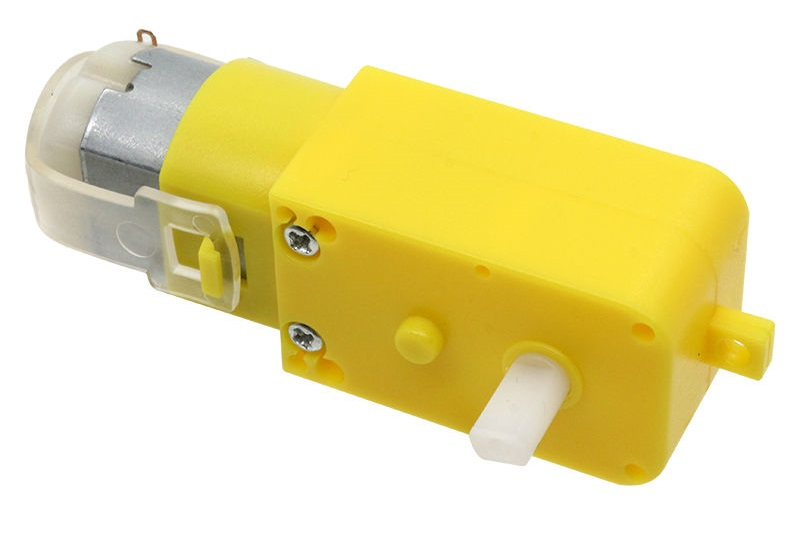
\includegraphics[width=8cm]{./Figures/Motorreductor.jpg}
	\caption{Imagen del motor utilizado\protect\footnotemark.}
	\label{fig:motorreductor}
\end{figure}
\footnotetext{Imagen tomada de \url{https://robots-argentina.com.ar/}}

Los motores elegidos cuentan con una caja de reducción (48:1) acoplada al eje del motor eléctrico, para lograr la disminución de velocidad, y un eje lateral que permite reducir espacio al utilizarlos en una configuración diferencial. La tensión nominal de trabajo va de los  3 a 6 V. Este modelo de motorreductor es ampliamente difundido en el mercado de componentes para robótica didáctica, por lo que es de fácil adquisición y bajo costo. 

En la tabla \ref{tab:caracteristicas} se referencian las principales características de los motores, según su tensión nominal de alimentación. 

\begin{table}[htpb]
\centering
\caption[características]{Características de los motores.}
\begin{tabular}{lccc}
                    & 3V DC       & 5V DC       & 6V DC      \\ \hline
Reducción           & \multicolumn{3}{c}{48:1}               \\
Velocidad sin carga & 125 RPM     & 200 RPM     & 230 RPM    \\
Velocidad con carga & 95 RPM      & 152 RPM     & 175 RPM    \\
Torque              & 0,8 kg.cm   & 1 kg.cm     & 1,1 kg.cm  \\
Corriente           & 110-130 mA  & 120-140 mA  & 130-150 mA \\
Dimensiones         & \multicolumn{3}{c}{70mm x 22mm x 18mm} \\
Peso                & \multicolumn{3}{c}{50g}                \\
Ruido               & \multicolumn{3}{c}{\textless{}65dB} 		\\  \hline
\end{tabular}
\label{tab:caracteristicas}
\end{table}


En la figura \ref{fig:planomoto} se pueden observar las dimensiones del motor utilizado.

%
\pagebreak

\begin{figure}[h]
	\centering
	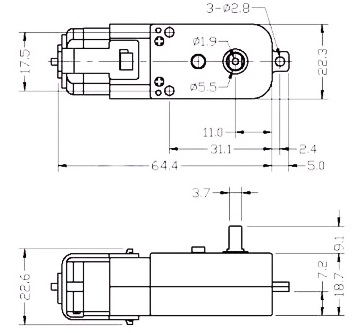
\includegraphics[width=10cm]{./Figures/planomoto.jpg}
	\caption{Dimensiones del motor utilizado\protect\footnotemark.}
	\label{fig:planomoto}
\end{figure}
\footnotetext{Imagen tomada de \url{https://robots-argentina.com.ar/}}

\subsection{Diseño del chasis y la carcasa del robot}
Se optó por una configuración de tracción de tipo diferencial \citep{traccion} que permite al robot girar sobre su propio eje. Se usan dos ruedas controladas individualmente junto con una rueda loca como tercer punto de apoyo. Esta configuración permite al robot moverse en espacios interiores y evitar obstáculos sin quedar atascado. 
Se construyó una base en acrílico para montar los motores y colocar encima las placas electrónicas de control y accionamiento del robot. En la figura \ref{fig:base} se muestra la base y la distribución física de los motores. 

\begin{figure}[h]
	\centering
	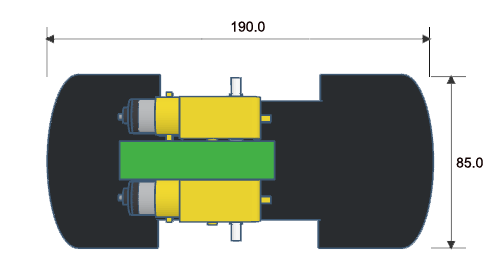
\includegraphics[width=11cm]{./Figures/base.png}
	\caption{Base y distribución de los motores.}
	\label{fig:base}
\end{figure}

Las dimensiones de esta base se determinaron en función de las dimensiones de los motores y de la placa principal de procesamiento. En la figura \ref{fig:baseeduciaa} se muestra la base en relación con la placa EDU-CIAA, ruedas y baterías. 

\begin{figure}[h]
	\centering
	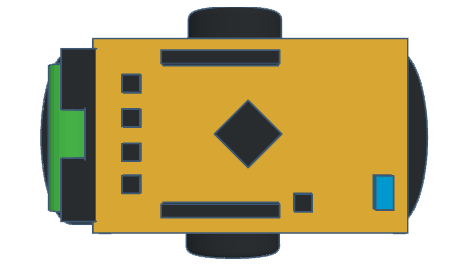
\includegraphics[width=9cm]{./Figures/baseeduciaa.png}
	\caption{Base y distribución de los motores.}
	\label{fig:baseeduciaa}
\end{figure}

El chasis se completa con una base circular sobre la que se integrarán los sensores y el resto de la carcasa. Esta forma responde a la necesidad de evitar que el robot quede atorado entre obstáculos (como pueden ser patas de mesas o sillas). La base circular sumada a la tracción diferencial permite al robot salir de cualquier encrucijada por el mismo camino por el que accedió, ya que puede rotar sobre sí mismo y no presenta irregularidades que puedan trabarse. En la figura \ref{fig:base2} se muestra la integración de la base inicial con el chasis circular. 

\begin{figure}[h]
	\centering
	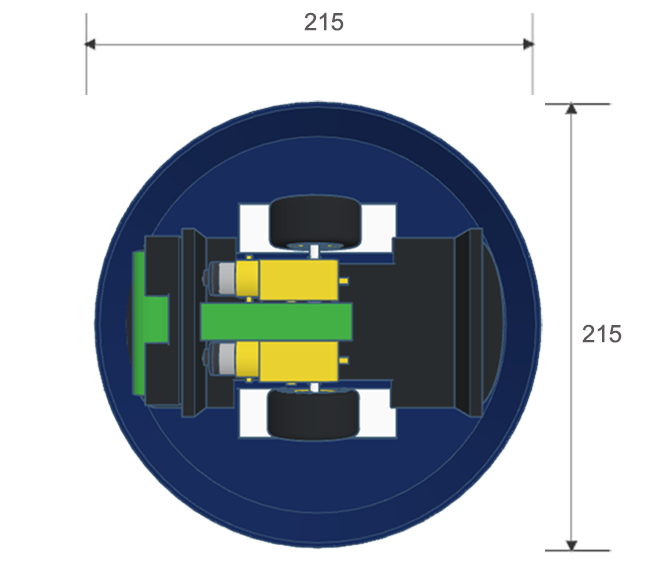
\includegraphics[width=12cm]{./Figures/base2.png}
	\caption{Base circular.}
	\label{fig:base2}
\end{figure}

En la figura \ref{fig:basearmada} se muestra una vista 3D  de la base y los componentesla principales (motores, ruedas, driver de motores, baterías t placas de control. 


\begin{figure}[h]
	\centering
	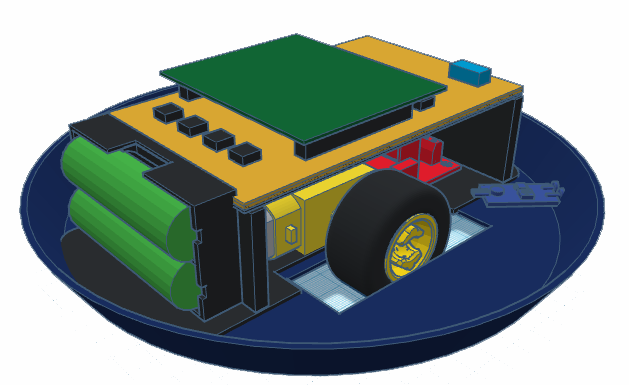
\includegraphics[width=11cm]{./Figures/basearmada.png}
	\caption{Modelo 3D de la base y componentes.}
	\label{fig:basearmada}
\end{figure}


\section{Diseño de hardware}

En esta sección se detallan los componentes y módulos electrónicos que forman parte del robot y se describe la función que desempeña cada uno de ellos. En la figura \ref{fig:diagramaini} se puede apreciar un diagrama en bloques de los módulos que conforman el robot.


\begin{figure}[h]
	\centering
	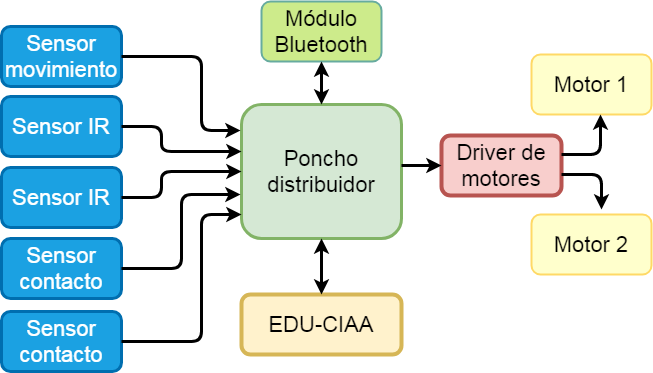
\includegraphics[width=12cm]{./Figures/diagini.PNG}
	\caption{Diagrama en bloques del robot.}
	\label{fig:diagramaini}
\end{figure}



	\subsection{Placa de expansión de hardware}
La denominación  “Poncho”  es utilizada dentro de la comunidad del proyecto CIAA para referirse a una placa de expansión o “shield” que se conecta sobre algún procesador de la familia CIAA.  
Para este trabajo se diseñó una placa de expansión de hardware con el fin de facilitar las conexiones de la placa EDU-CIAA con los sensores, actuadores y el módulo de comunicación bluetooth.

	\subsubsection{Diseño esquemático de la placa de expansión de hardware}

La placa de expansión de hardware presenta varios conectores para simplificar en conexionado de los distintos sensores, ya que varios de ellos requieren no solo ser cableados a un determinado pin de la placa EDU-CIAA, sino que ademas necesitan conexión a las líneas de alimentación. Los conectores corresponden a los siguientes sensores / señales de entrada:

\begin{itemize}
	\item Sensores infrarrojos (2).
	\item Finales de carrera (2).
	\item Sensor de movimiento (1).
	\item Pulsador de cambio de modo (1).
	
\end{itemize}

La elección de los puertos utilizados para la atención de cada sensor contempló la distancia entre pines de modo de optimizar el ruteo de la placa. En la figura \ref{fig:consesnores} se observa detalle de cada  conector en la placa de expansión con los puertos de la EDU-CIAA.


\begin{figure}[h]
	\centering
	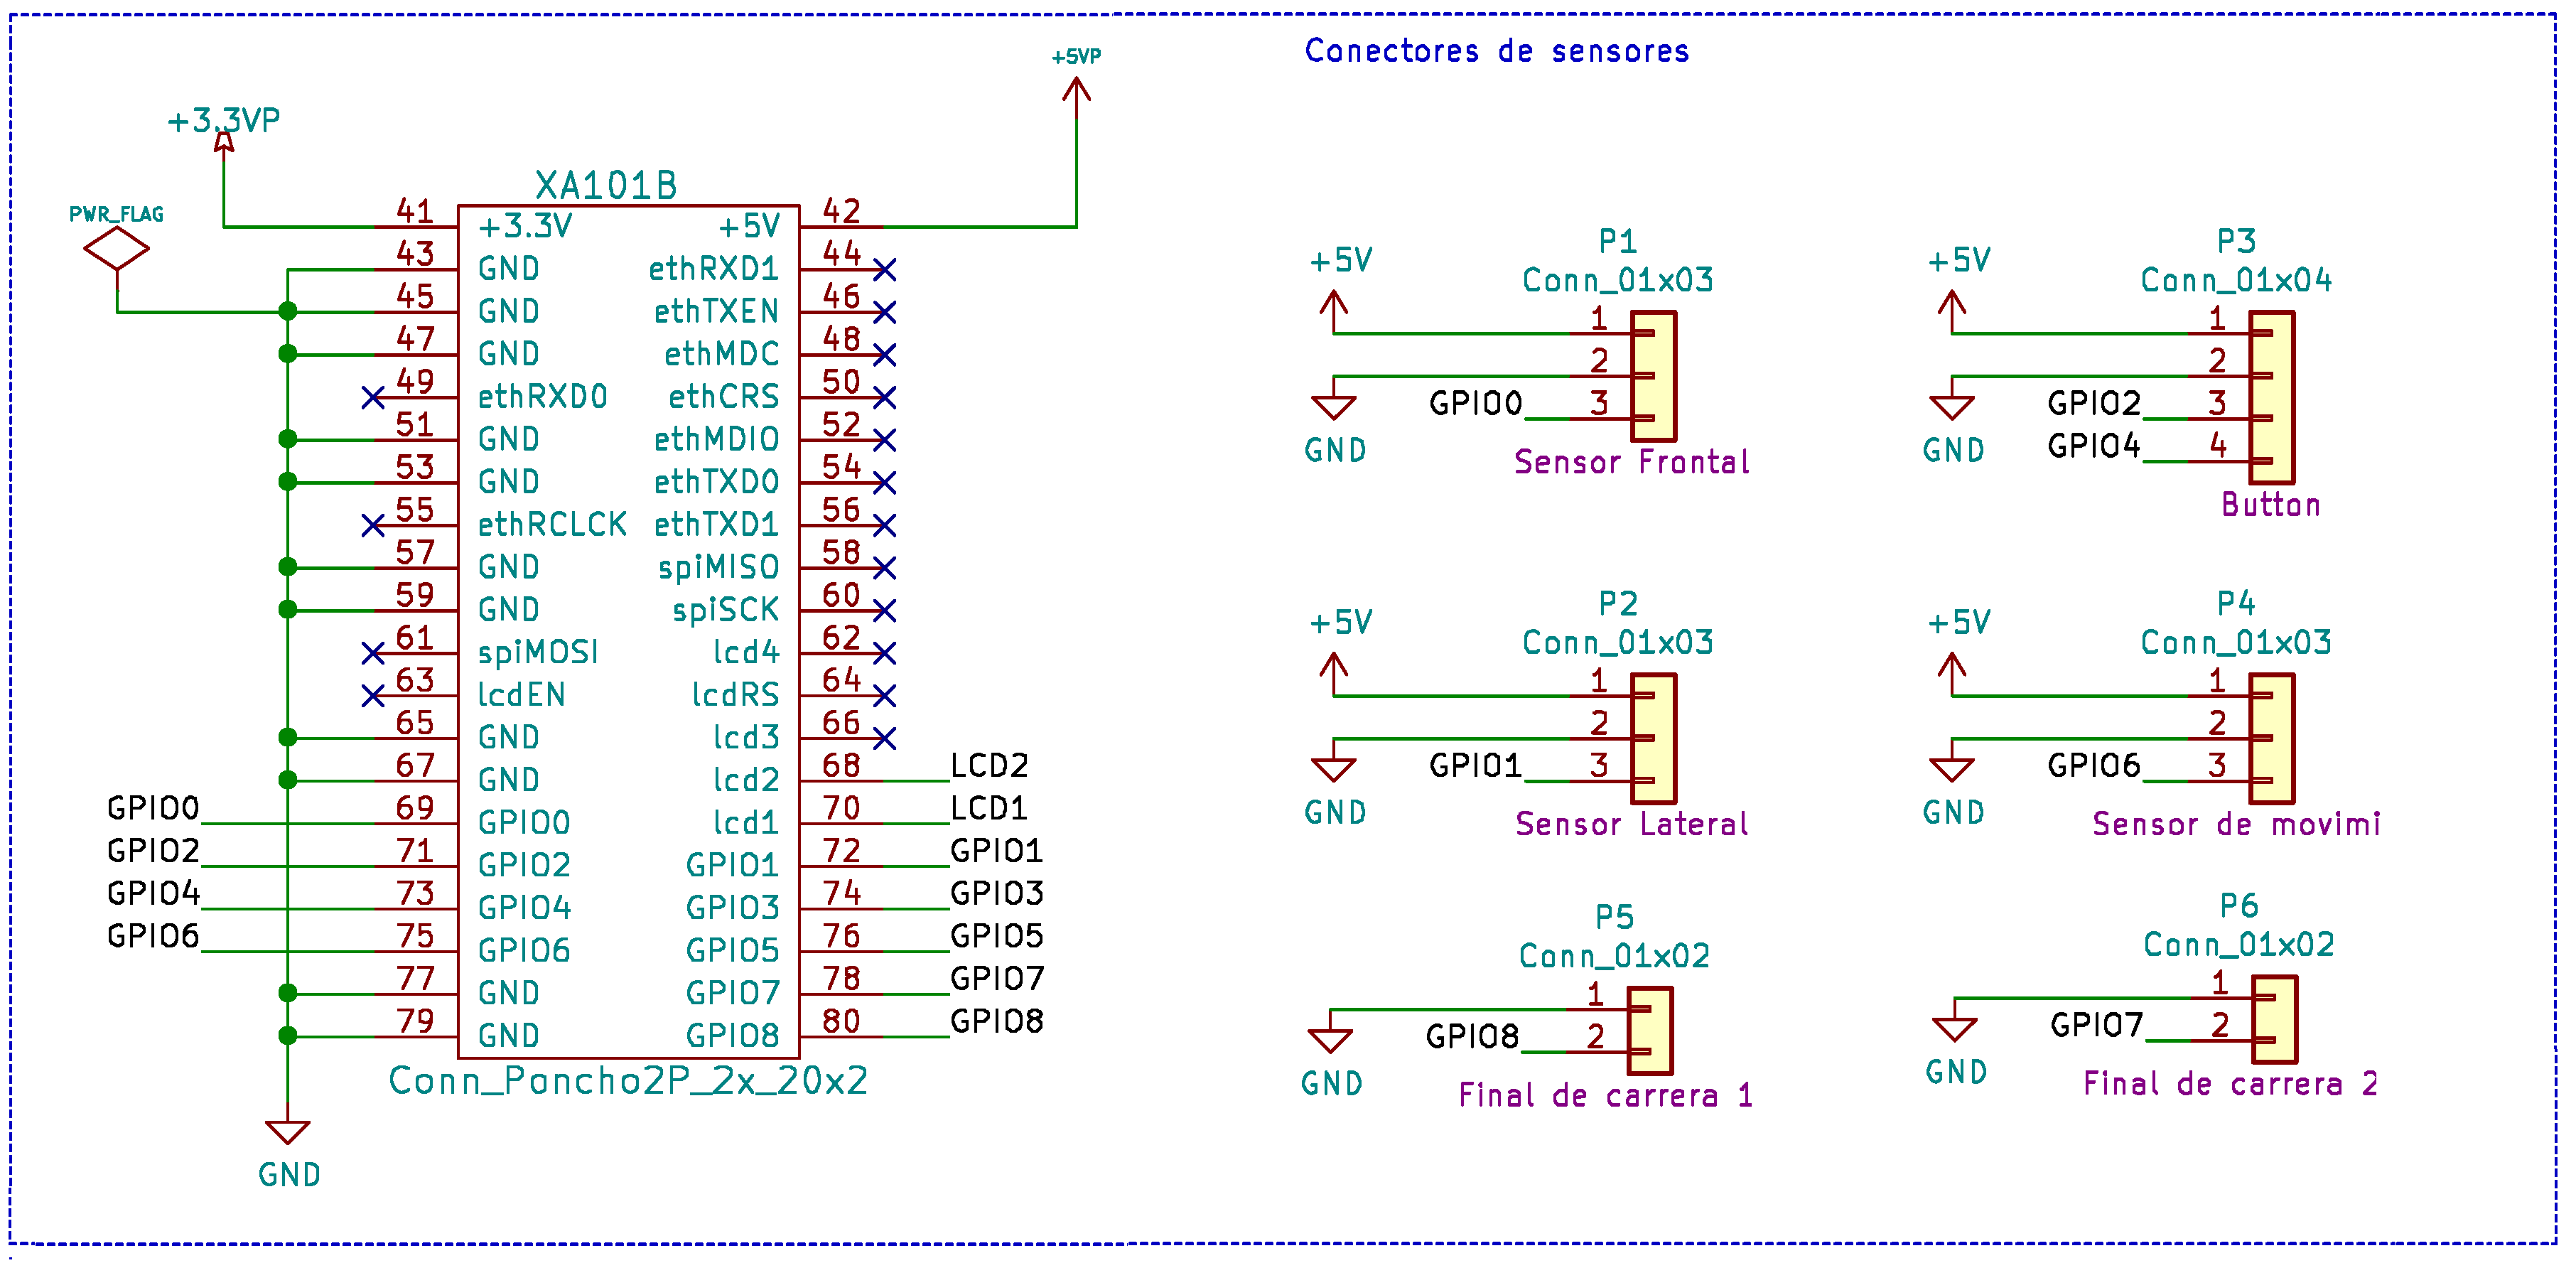
\includegraphics[width=13cm]{./Figures/sensores2.PNG}
	\caption{Esquemático de conexionado de sensores.}
	\label{fig:consesnores}
\end{figure}

La placa de expansión permite también la conexión con el módulo de control de motores, como dispositivo de salida, y conecta con los siguientes actuadores integrados en la placa:

\begin{itemize}
	\item Relé actuador.
	\item Buzzer
	\item LED indicador de alimentación.
	\item LED indicador de relé encendido.
\end{itemize}


El relé se utiliza para activar o desactivar dispositivos conectados a la bornera de la placa, de modo que los mismos puedan contar con una alimentación independiente. En el caso particular de la presente aplicación el relé permite conmutar el modulo de luz ultravioleta germicida. 
La utilización del relé permite no solo la aislación eléctrica del circuito de control con el dispositivo a controlar, sino que habilita también la posibilidad de intercambiar el módulo UVC por otro de distintas características. Por ejemplo, se podría utilizar otro tipo de lámpara UVC con su propia alimentación.  
En la figura \ref{fig:rele} se muestra el conexionado del relé y su bornera.

\begin{figure}[h]
	\centering
	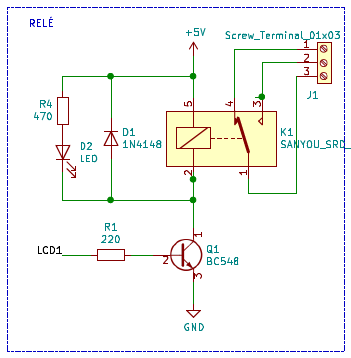
\includegraphics[width=7cm]{./Figures/rele.PNG}
	\caption{Esquemático de conexionado del relé.}
	\label{fig:rele}
\end{figure}


El buzzer aporta señalización sonora sobre el estado de operación del robot. Se utilizó un Buzzer Activo que  posee su propia
frecuencia de oscilación. Al presionar el pulsador (en forma demorada) se producen dos pitidos que indican el paso del modo teleoperado al modo autónomo, y un pitido al realizar el paso inverso. En la figura \ref{fig:buzzer} se observa el conexionado del buzzer por medio de un transistor.

\begin{figure}[h]
	\centering
	\includegraphics[width=5cm]{./Figures/buzzer.PNG}
	\caption{Esquemático de conexionado del buzzer.}
	\label{fig:buzzer}
\end{figure}
%%
%\pagebreak

La placa posee un zócalo para el conexionado del módulo  de comunicación bluetooth (HC-05) y otro zócalo destinado a dispositivos I2C (como podría ser un módulo de giróscopo o acelerómetro). El módulo bluetooth permite la comunicación con el dispositivo externo (teléfono celular o Tablet) para el modo de operación remoto. El módulo se conecta directamente sobre la placa, para evitar cables y por lo tanto, la posibilidad de ruido en la conexión. También resulta conveniente para reducir el espacio del montaje. 
En la figura \ref{fig:conectorbt} se observa un detalle del conexionado en la placa para el módulo Bluetooth HC-05 y cualquier dispositivo I2C.


\begin{figure}[h]
	\centering
	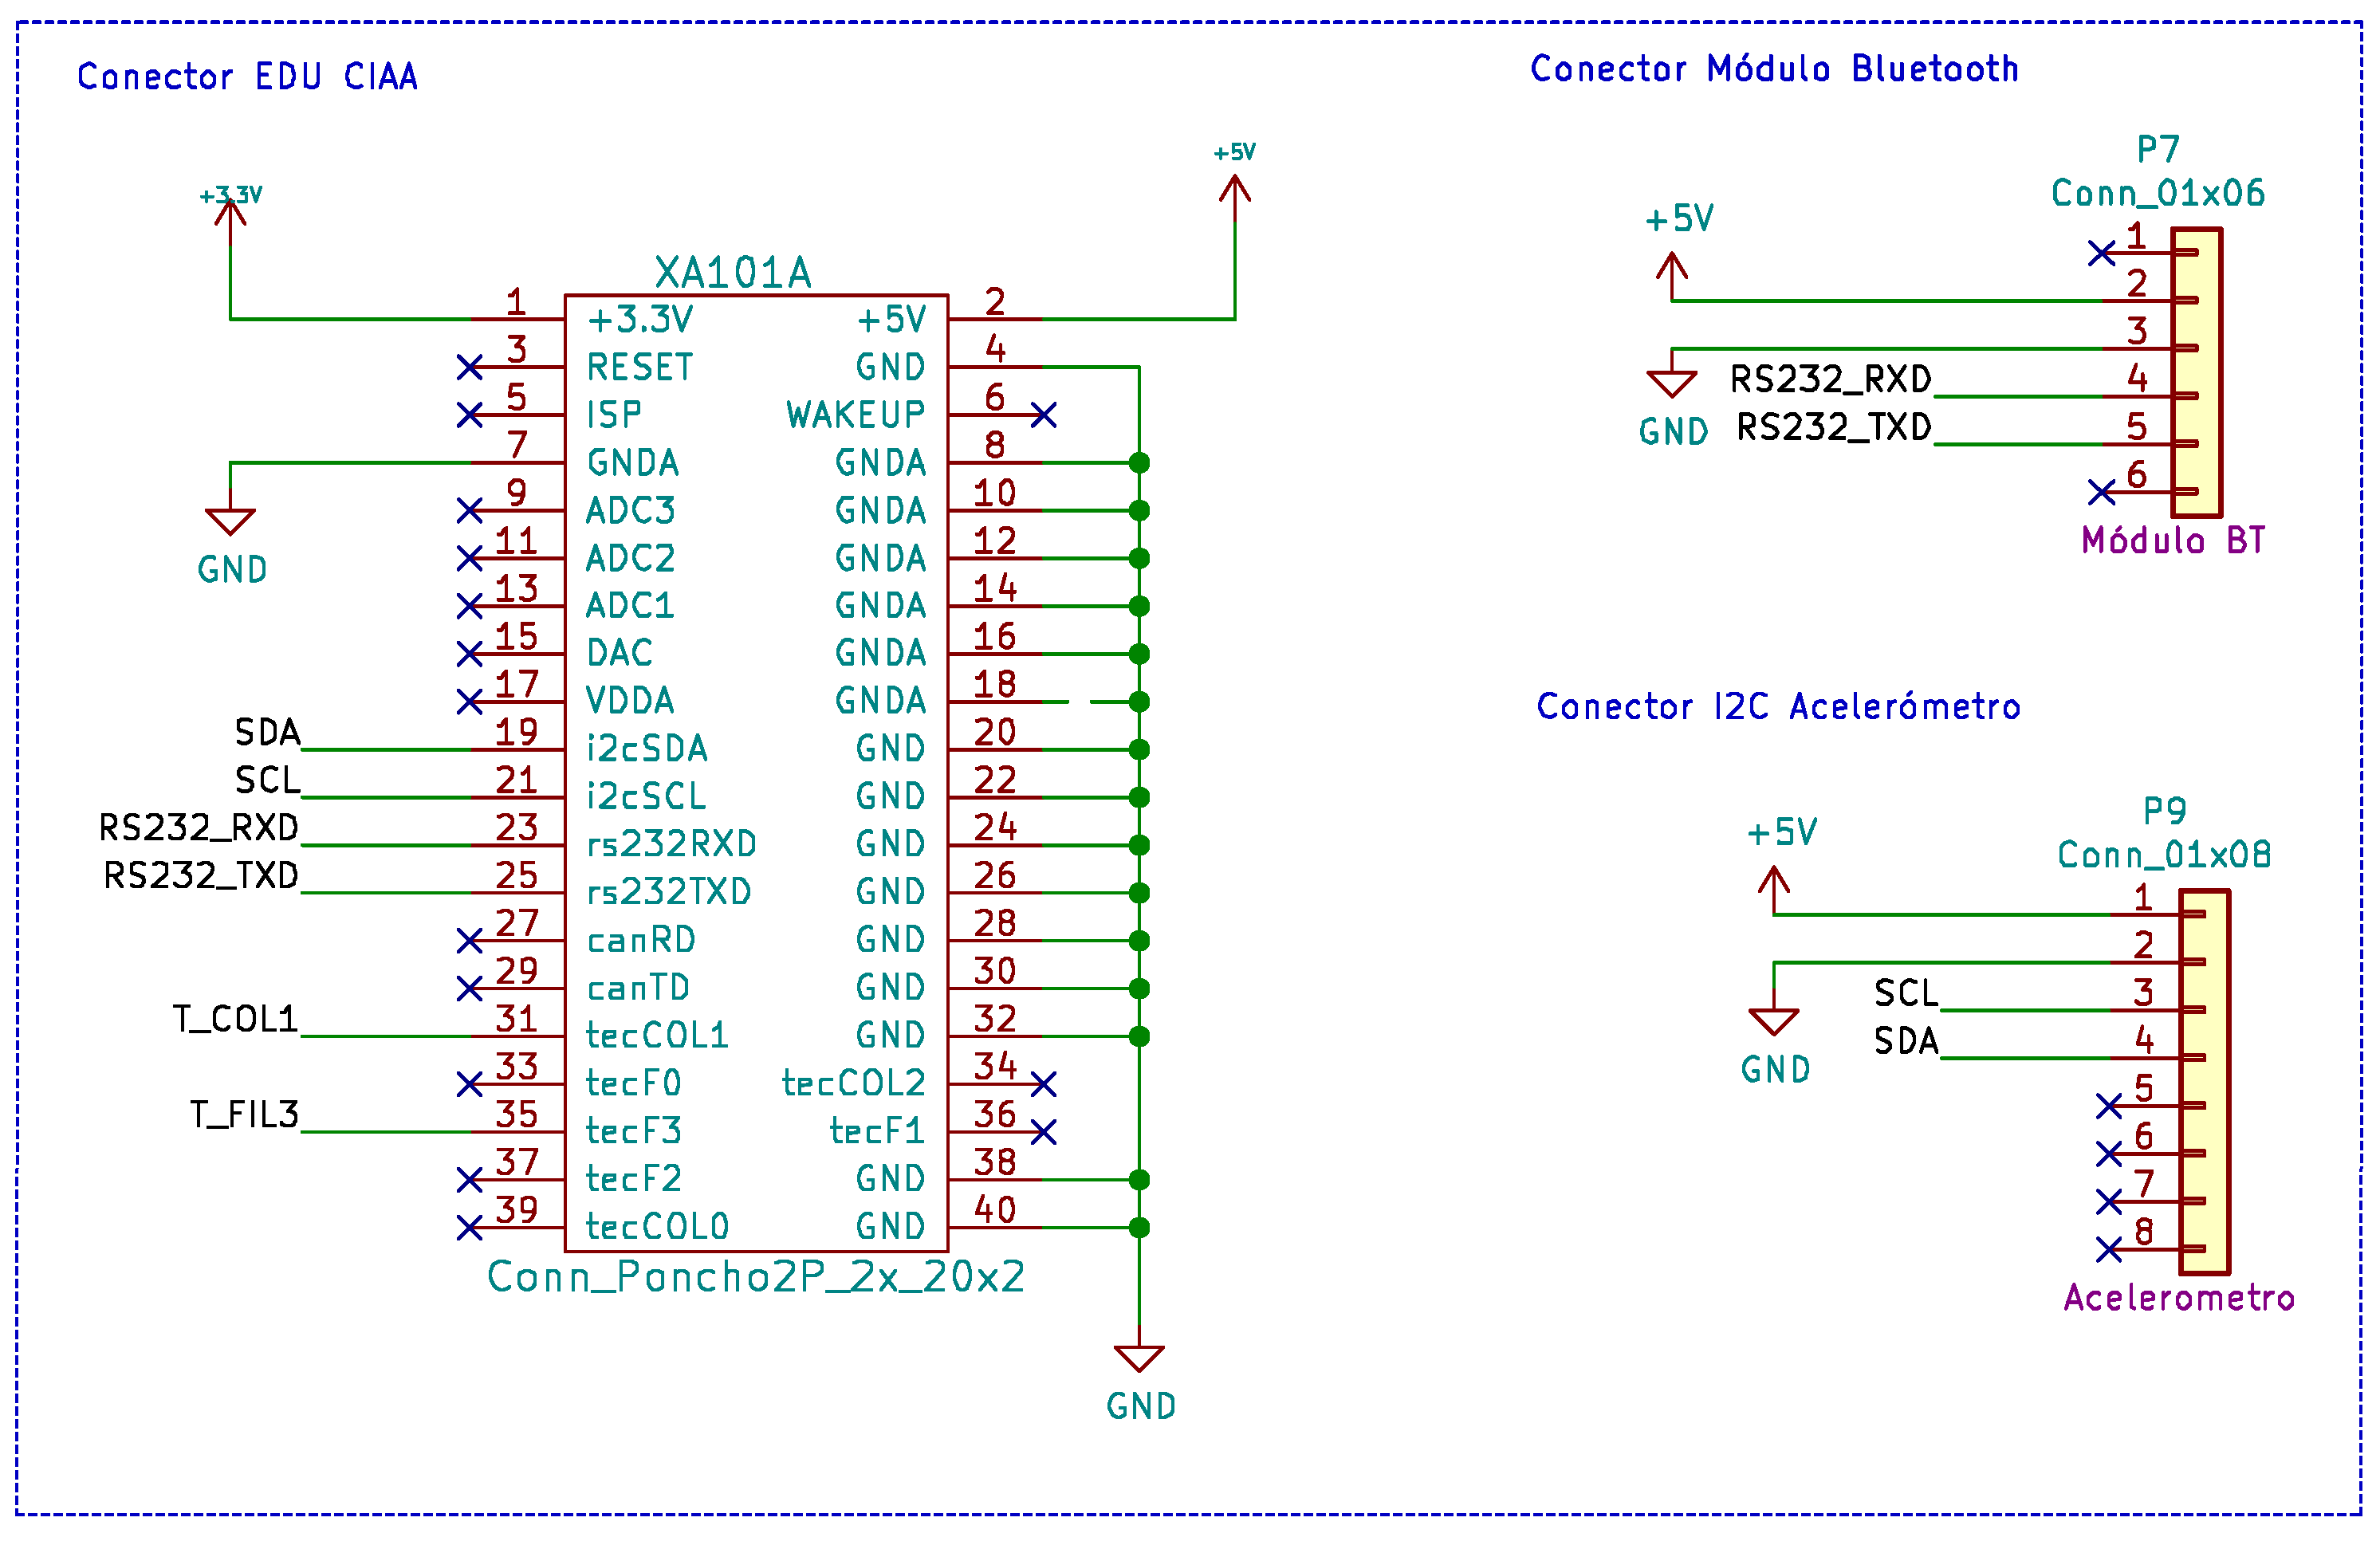
\includegraphics[width=13cm]{./Figures/conectorbt2.PNG}
	\caption{Conectores para los módulos Bluetooth e I2C.}
	\label{fig:conectorbt}
\end{figure}



		\subsubsection{Diseño PCB de la placa de expansión de hardware}


La placa fue diseñada durante la cursada de la asignatura “diseño de circuitos impresos", según los lineamientos expuestos en la documentación para placas de expansión de hardware para la EDU-CIAA. 

El diseño de PCB se realizó con el software KiCad \citep{KiCad} (Versión 5.1.9), el cual es un paquete de software para el diseño de circuitos electrónicos o EDA (Electronic Design Automation). En la figura \ref{fig:poncho3d} se observa el modelo 3D de la placa y sus componentes. 

\begin{figure}[h]
	\centering
	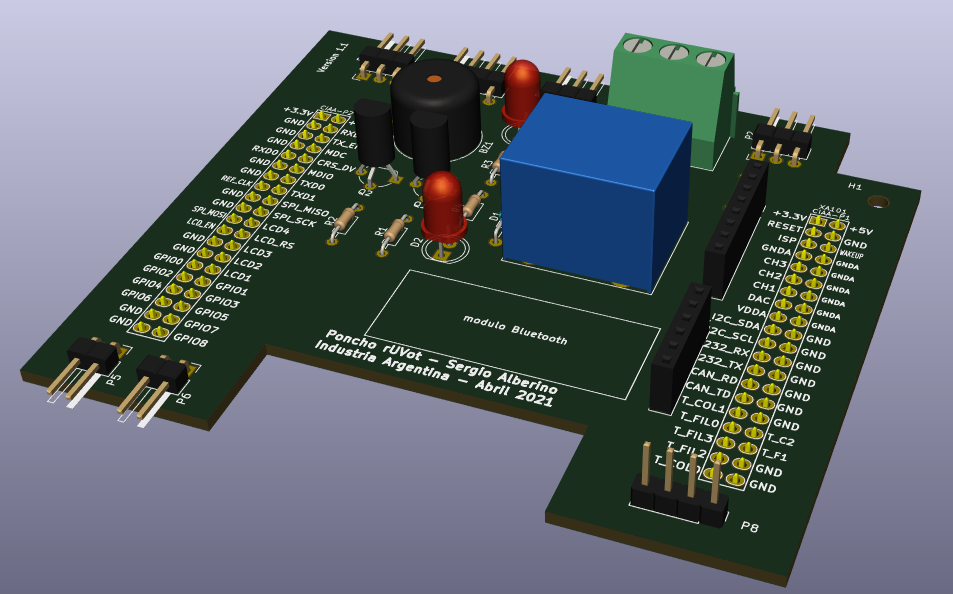
\includegraphics[width=11cm]{./Figures/ponchoiso.PNG}
	\caption{Vista del modelo 3D de la placa de expansión de hardware.}
	\label{fig:poncho3d}
\end{figure}

\pagebreak

Una vez completado y validado el diseño, se generaron los archivos de fabricación para su procesado con técnicas caseras. 
En la figura \ref{fig:placafoto1} se puede observar una  imagen de la placa procesada, con sus componentes soldados y el módulo Bluetooth insertado en el conector correspondiente.


\begin{figure}[h]
	\centering
	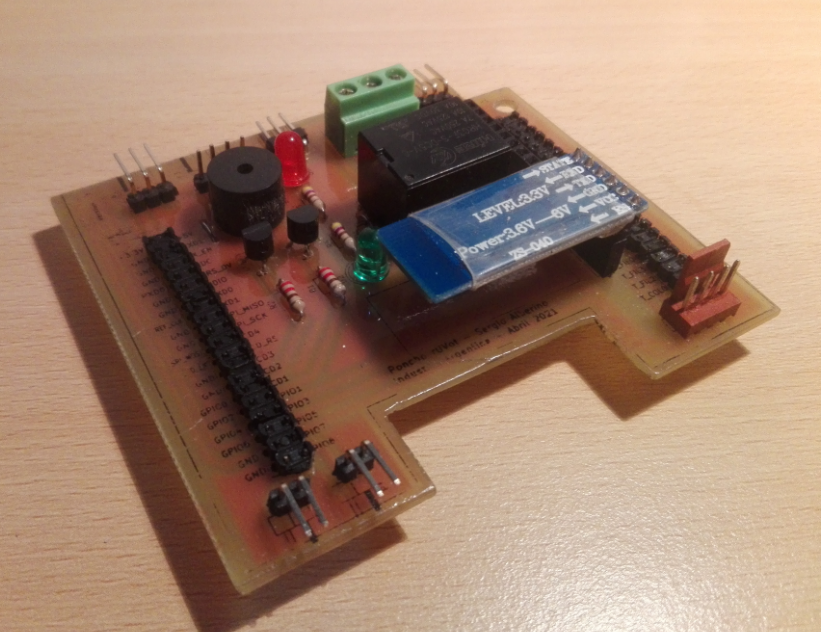
\includegraphics[width=11cm]{./Figures/placafoto.png}
	\caption{Fotografía de la placa desarrollada.}
	\label{fig:placafoto1}
\end{figure}

		\subsubsection{Conexionado para motores}

Para el accionamiento de los motores se utilizó modulación por ancho de pulsos (PWM, por su sigla en inglés). La placa EDU-CIAA posee un solo modulo PWM con 11 salidas asociadas. Todas las salidas PWM comparten la misma frecuencia, aunque puede asignarse un valor de ciclo de actividad en forma independiente.

\begin{itemize}
	\item PWM0:  GPIO\_2.
	\item PWM1:  GPIO\_8.
	\item PWM2:  T\_FIL1.
	\item PWM3:  T\_FIL2.
	\item PWM4:  T\_FIL3.
	\item PWM5:  T\_COL0.
	\item PWM6:  T\_COL1.
	\item PWM7:  T\_COL2.
	\item PWM8:  LCD\_1.
	\item PWM9:  LCD\_2.		
	\item PWM10: LCD\_3.				
\end{itemize}

Se utilizaron las líneas de T\_FIL3: PWM4 y T\_COL1: PWM6 para el control de los motores.



		\subsubsection{Disposición de Entradas y Salidas}

Se utilizaron los pines de entrada/salida de Propósito General (GPIO, General Purpose Input/Output)de la placa Edu-CIAA para el conexionado de sensores y actuadores. El módulo GPIO de la sAPI permite modelar un único pin de entrada/salida o un puerto completo.
Los pines utilizados son:

\begin{itemize}
	\item GPIO0:  	Sensor IR frontal.
	\item GPIO1:  	Sensor IR lateral.
	\item GPIO2:  	Pulsador externo.
	\item GPIO3:  	Dirección motor.	
	\item GPIO4:  	Señalización Pulsador.
	\item GPIO5:  	Dirección motor.		
	\item GPIO6:  	Sensor PIR. 
	\item GPIO7:  	Sensor de contacto. 
	\item GPIO8:  	Sensor de contacto. 
	\item LCD\_1:  	Relé.
	\item LCD\_2:  	Buzzer.		
\end{itemize}


%\begin{figure}[h]
%	\centering
%	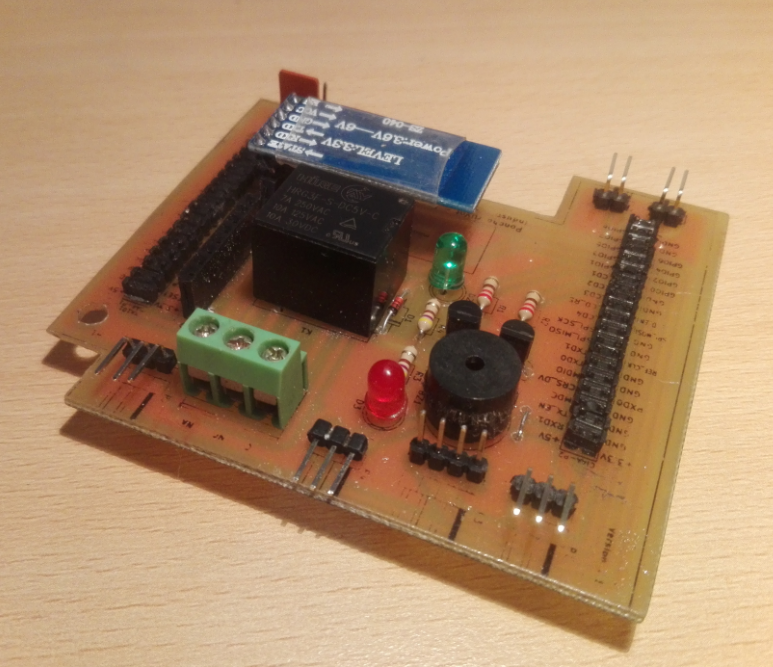
\includegraphics[width=11cm]{./Figures/placafoto2.png}
%	\caption{Fotografía de la placa desarrollada.}
%	\label{fig:placafoto2}
%\end{figure}



%@book{traccion,
%	author={Secchi, Humberto Alejandro},
%	title={Una introducción a los robots móviles},
%    PUBLISHER="AADECA. Buenos Aires (Argentina)",
%	year={2008}
%}


%presenta el circuito esquemático del poncho donde se puede observar el conexionado eléctrico.

%\begin{figure}[h]
%	\centering
%	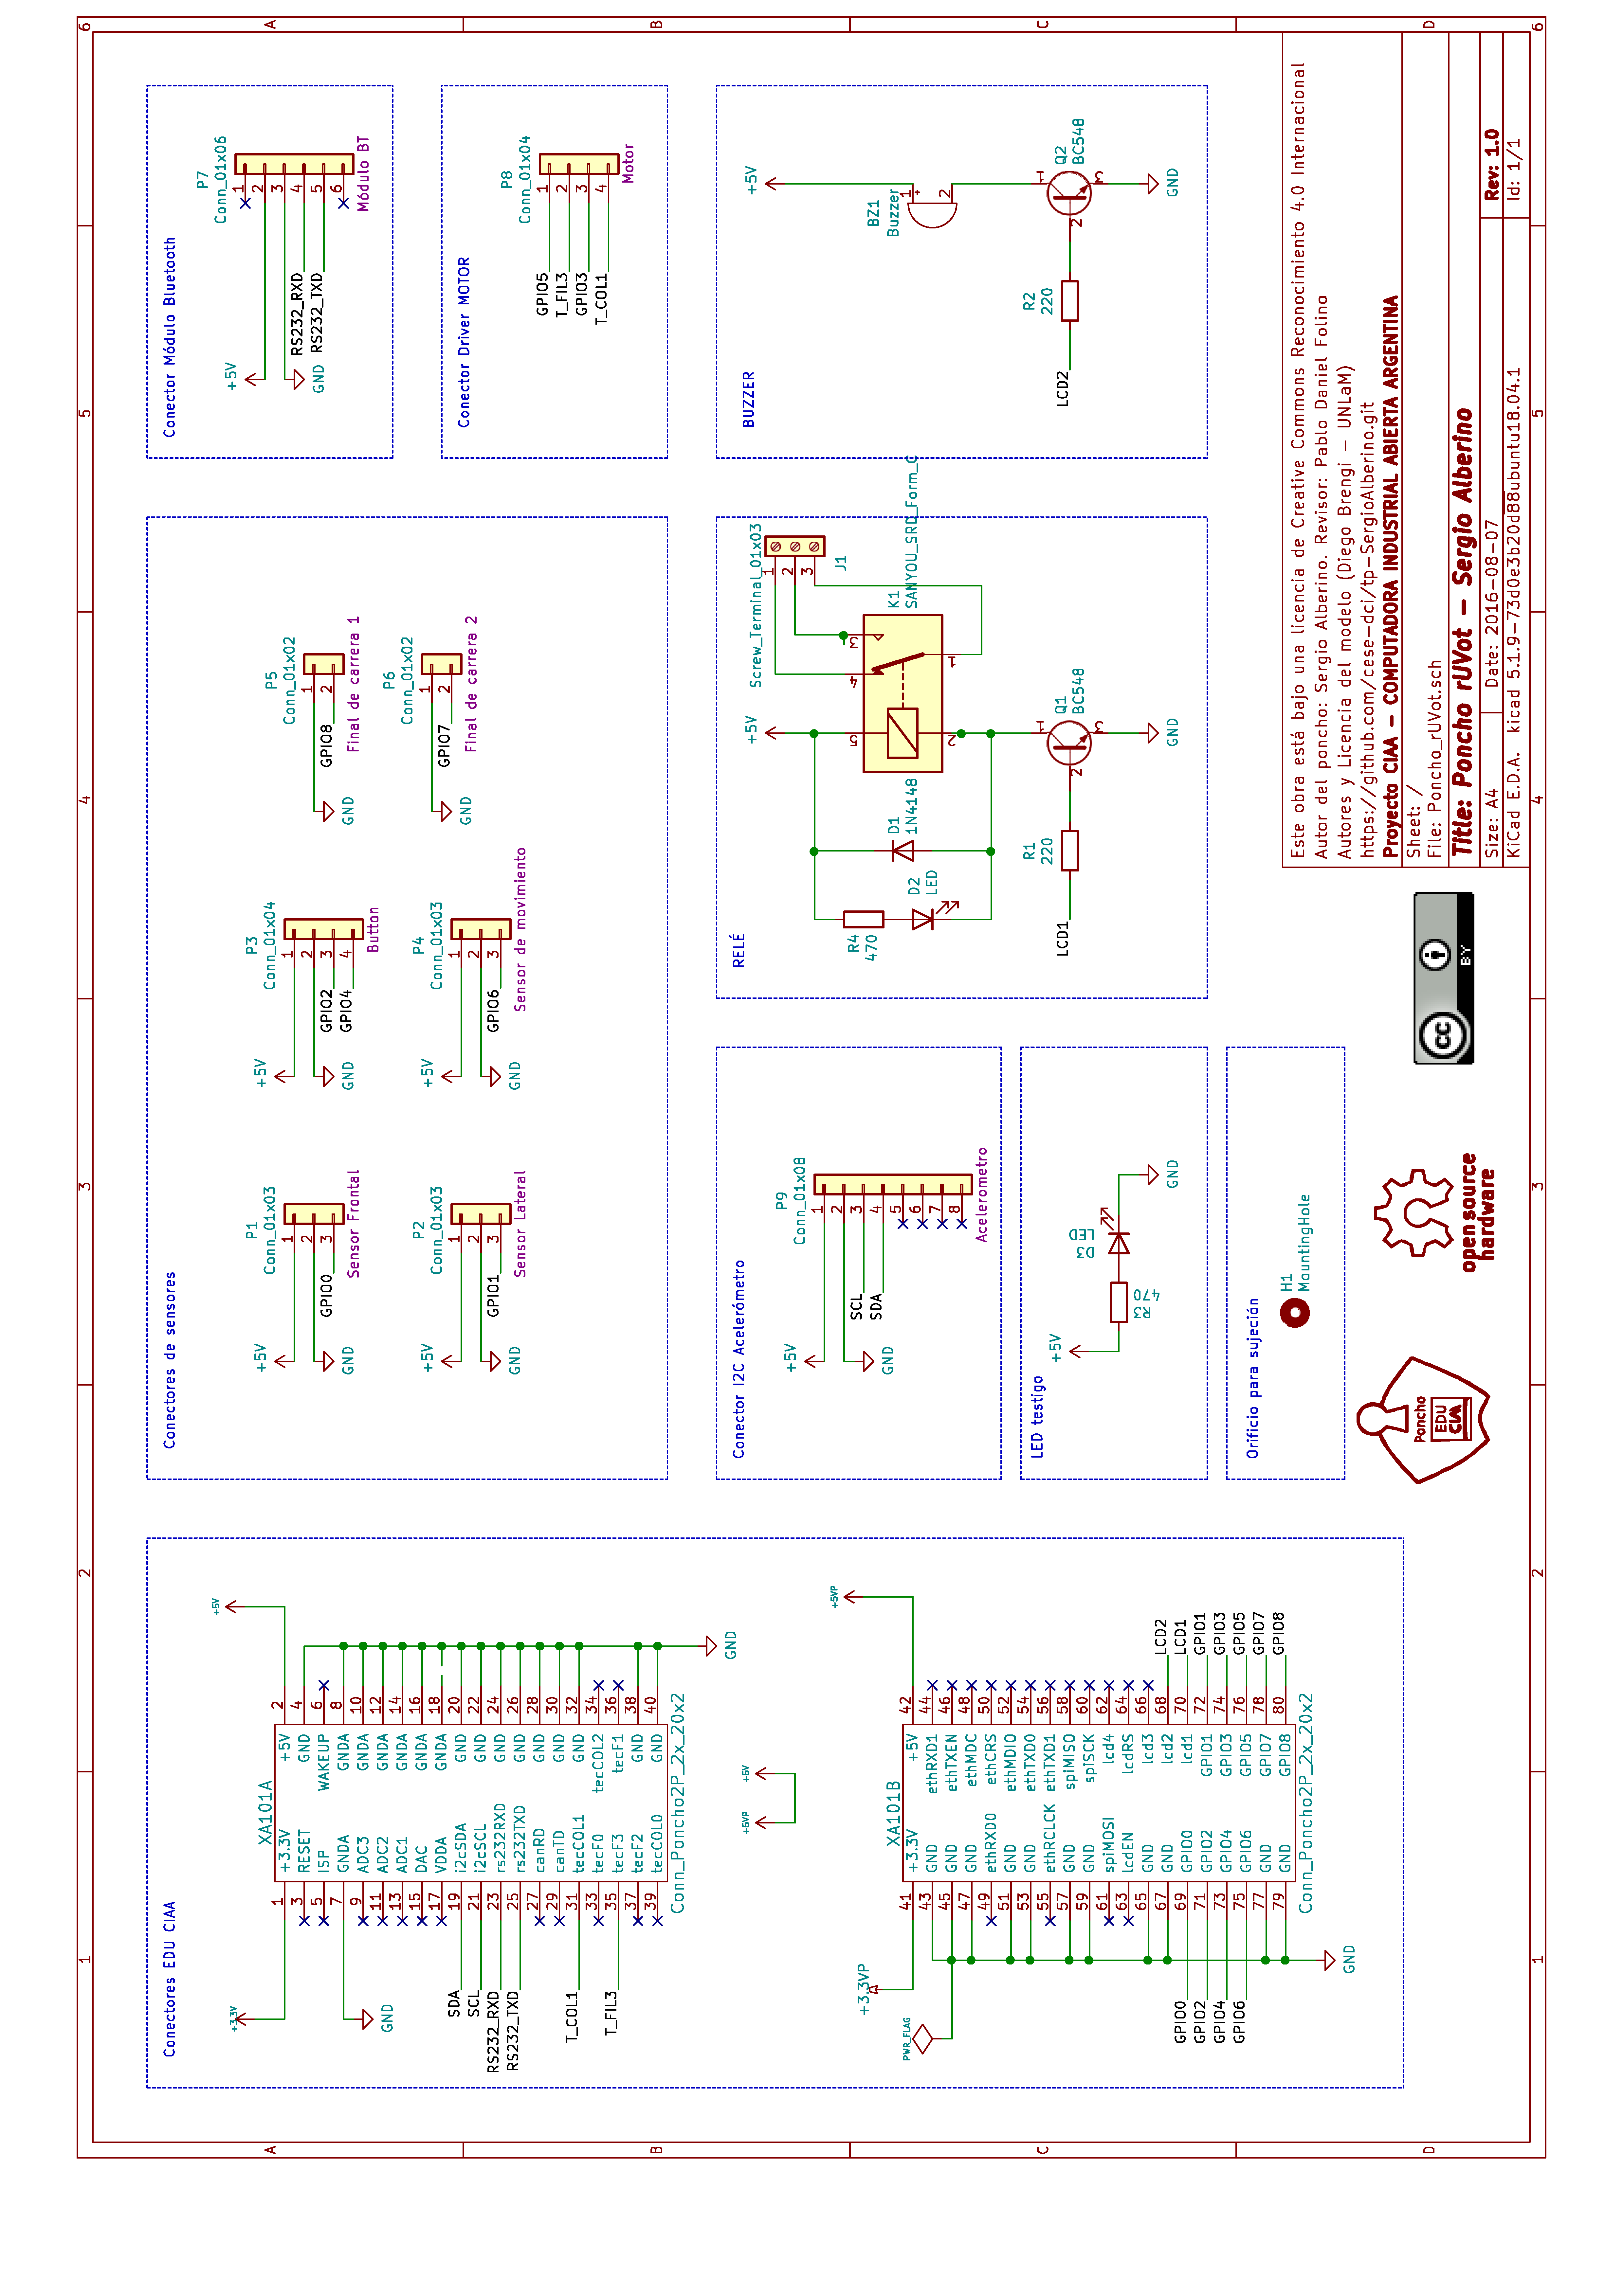
\includegraphics[width=\textwidth]{./Figures/esquematico.png}
%	\caption{Circuito esquemático del poncho.}
%	\label{fig:esquematico}
%\end{figure}
%\pagebreak

%\subsection{Esquema de  de comunicaciones}


\section{Diseño de software}

Para la arquitectura del firmware se tuvo en cuenta un patrón de diseño de arquitectura de control ambiental \citep{arq}, ya que se trata de un patrón de control general que incluye procesos de sensor y actuador, y es el que más se acerca al modelo de comportamiento del robot.
La programación se realizó utilizando lenguaje C sobre el firmware de la EDU-CIAA versión 3 como capa de abstracción de hardware. 
Se utilizaron módulos de software de la biblioteca sAPI para acceder de manera simple a los diferentes periféricos.
Se modularizó el firmware en archivos, de modo de mantener en un mismo módulo de software las instrucciones relacionadas con cada periférico y que puedan utilizarse (y reutilizarse) en forma ordenada. 
Se utilizó una máquina de estados finitos como rutina principal para el comportamiento autónomo del robot, en función reactiva a la información obtenida por los sensores.

%
%\subsection{Estructura de capas}
El diseño del firmware se organizó como una estructura de capas, lo cual permite la separación de las partes que componen el sistema.

\subsection{Módulos de software}

		\subsubsection{Máquina de estados finitos}
Las Máquinas de Estado Finitas (FSM, por su sigla en inglés) son utilizadas ampliamente como rutinas para reconocimiento de secuencias de datos, para interpretación de tramas de comunicación serie, y para el ordenamiento de tareas ante distintas condiciones medidas. Son básicamente estructuras de programa cuyo comportamiento está determinado por el “estado” en el que se encuentran y por variables (generalmente booleanas) de entrada, ofreciendo para cada caso una salida y un “estado próximo” (que puede tratarse del mismo estado en el que se encuentra).
El uso de FSM es sencillo, implica un bajo consumo de procesamiento, y resulta flexible para el agregado de nuevas condiciones y estados. Sin embargo, cuando el número de entradas crece, su implementación y mantenimiento puede resultar complejo ya que el comportamiento se establece en el código fuente.

Se utilizó un método en el que la máquina de estados se actualiza a partir de los datos registrados en  una estructura de datos de estados/entradas/salidas almacenada en un archivo header en la memoria del microcontrolador (MdE.h). Las variables de entrada son de tipo booleano y las acciones planteadas por la tabla corresponden a comportamientos puramente reactivos. La solución ha sido presentada en un trabajo de investigación anterior \citep{planilla}.

La ventaja del método utilizado radica en el uso de una aplicación que permite generar el contenido del archivo header a partir de una hoja de cálculo en la que se pueden consignar las distintas acciones a partir de las combinaciones de estado actual y condiciones de entrada. En la planilla de configuración, es posible “enmascarar” condiciones que son indiferentes al comportamiento  usando el valor “X” (interpretado semánticamente como “indeterminado”), que luego es expandido por la aplicación intérprete de modo que finalmente en la estructura de datos de la FSM se consideren todas las condiciones como valores booleanos. 
La aplicación verifica que no se produzcan combinaciones redundantes o inválidas y se encarga de construir el archivo header con la estructura ordenada de datos para la actualización de la FSM,  para ser transferido al microcontrolador del robot.

La FSM se implementa como rutina principal, tomando los datos de la tabla procesada y consignada en el archivo header, y partiendo siempre de un Estado Inicial. La rutina de la FSM utiliza pocos recursos de procesamiento, relevando las variables de entrada y el valor del Estado actual, y localizando en la tabla la opción de salida y el Estado al que debe pasar .
		
		
		
		\subsubsection{Sensores}
		\subsubsection{Motores}


\subsection{Herramientas de usuario}





Herramientas de usuario



%
%
%
%
%\begin{verbatim}
%\begin{lstlisting}[caption= "un epígrafe descriptivo"]
%	las líneas de código irían aquí...
%\end{lstlisting}
%\end{verbatim}
%
%A modo de ejemplo:
%
%\begin{lstlisting}[label=cod:vControl,caption=Pseudocódigo del lazo principal de control.]  % Start your code-block
%
%#define MAX_SENSOR_NUMBER 3
%#define MAX_ALARM_NUMBER  6
%#define MAX_ACTUATOR_NUMBER 6
%
%uint32_t sensorValue[MAX_SENSOR_NUMBER];		
%FunctionalState alarmControl[MAX_ALARM_NUMBER];	//ENABLE or DISABLE
%state_t alarmState[MAX_ALARM_NUMBER];						//ON or OFF
%state_t actuatorState[MAX_ACTUATOR_NUMBER];			//ON or OFF
%
%void vControl() {
%
%	initGlobalVariables();
%	
%	period = 500 ms;
%		
%	while(1) {
%
%		ticks = xTaskGetTickCount();
%		
%		updateSensors();
%		
%		updateAlarms();
%		
%		controlActuators();
%		
%		vTaskDelayUntil(&ticks, period);
%	}
%}
%\end{lstlisting}



